\documentclass[12pt, a4wide]{scrreprt}
\usepackage{scrhack}
\usepackage{scrpage2}
\usepackage{graphicx}
\usepackage[utf8]{inputenc}
\usepackage{ngerman}
\usepackage{multicol}
\usepackage[printonlyused,withpage]{acronym}

\usepackage{titlesec}

%numbers braucht man wohl für IEEEtranN
\usepackage[numbers]{natbib}

%irgendein hack für die Seitennummerierug-----v
\usepackage{tikzpagenodes}
\usetikzlibrary{calc}
\usepackage[contents={}]{background}


\begin{document}
\setkomafont{disposition}{\normalcolor\bfseries}
%-------Titelseite-------%
\noindent
Konstantin Obermann \hfill Mat.nr: 947545\\
Universität Osnabrück \hfill 23.10.2015\\
Wintersemester 15/16\\
\thispagestyle{empty}
\begin{center}

\includegraphics[scale=.9]{uos_proper.png}
\section*{}
{\LARGE Ausarbeitung zum Thema}\\
\section*{}
{\Huge {\bf Lokalisierung in drahtlosen Sensornetzwerken}}\\
\section*{}
{\Large Im Rahmen des Seminars ''Verteilte Systeme''}\\
\section*{}
{\Large Betreuer:}\\
{\Large Prof.Dr.rer.nat Nils Aschenbruck}\\
{\Large Dipl.-Inform. Matthias Schwamborn}\\
\end{center}


\newpage
\thispagestyle{empty}
\section*{Abkürzungsverzeichnis}
 \begin{acronym}
\acro{WSN}{Wireless Sensor Network}
\acro{AOA}{Angle of Arrival}
\acro{RSS}{Received Signal Strength}
\acro{TOA}{Time of Arrival}
\acro{TDOA}{Time Difference of Arrival}
\acro{COTS}{Commercial Off-The-Shelf}
\end{acronym}

\newpage
\newcommand{\myfooterstyle}[2][]{%
\tikz[remember picture,overlay]{%
   \draw[#1]
   ($(current page footer area.south west)!0.25!(current page footer area.north west)$)
   --
   ($(current page footer area.south)!0.25!(current page footer area.north)-(#2,0)$)
   ($(current page footer area.south)!0.25!(current page footer area.north)+(#2,0)$)
   --
   ($(current page footer area.south east)!0.25!(current page footer area.north east)$)
   ;
  }%
}

\AddEverypageHook{%
\myfooterstyle{1em}
\BgMaterial}
%--------------------------------------------^

%-----------Inhaltsverzeichnis--------------%
\tableofcontents
\pagenumbering{roman}


%-------Einleitung-------%
\chapter{Einleitung und Motivation}
\pagenumbering{arabic}
Der technologische und wirtschaftliche Fortschritt erfordert eine zuverlässige, konsistente und in vielen Fällen drahtlose Kommunikation. Beispiele für drahtlose Netzwerke sind Mobilfunknetzstandards GSM, UMTS und LTE oder das drahtlose Netzwerkprotokoll WLAN.

Das \ac{WSN} dagegen ist ein Netz aus Sensoren. Die besondere Eigenschaft dieser Sensoren ist, dass sie sehr klein sind, auf kurze Distanzen miteinander kommunizieren, sowie Daten verarbeiten können und sparsam im Energieverbrauch sind. Besonders die Fähigkeit, ein Ad-hoc-Netz aufzuspannen, macht die \acs{WSN} zu einem vielfältig einsetzbaren drahtlosen Netzwerk.

Die Herausforderung beim Einsatz der \acs{WSN} besteht in der richtigen Konfiguration und Ausstattung der Sensoren. Aufgrund ihrer geringen Größe bieten sie nur wenig Platz für Arbeitsressourcen(RAM, CPU), weshalb der Aufbau des WSN sorgfältig geplant werden sollte. Die bereits erwähnte Fähigkeit, automatisch ein Ad-hoc-Netz einzurichten, setzt voraus, dass sich die Knoten in einem Netzwerk \textit{selbstständig} finden können.

Diese Lokalisierung der einzelnen Sensorknoten erfolgt auf Basis von \ac{AOA}, \ac{RSS} oder distanzbasierten Ansätzen zur Positionsbestimmung. Eine schnelle Lokalisierung der einzelnen Sensoren erfolgt dann, wenn diese vorher optimal platziert werden, um die Anzahl an Knoten im WSN zu minimieren und den Overhead in den Lokalisierungsalgorithmen zu vermeiden\cite{area_based}.

Faktoren, wie Schnelligkeit und Präzision der Lokalisierung sowie der Grad der Autonomie des WSN, beeinflussen dessen Zuverlässigkeit und Potential. Dieses Potential ist entscheidend für die Auswahl der Einsatzmöglichkeiten. Das Erdbeben-Frühwarnsystem (EEW) ist eine der Anwendungsmöglichkeiten der \ac{WSN}. Hier ist eine reibungslose und schnelle Kommunikation zwischen den Knoten besonders wichtig, denn ein Fehlalarm ist kostspielig. Allerdings ein im Ernstfall verspäteter Alarm kann Menschenleben kosten. Weitere Beispiele für die Verwendung von Sensornetzen sind Erkennung von Waldbränden, Überwachung von Deichen, Überwachung von Gebäudestatik, um Erdbebenschäden zu erkennen\cite{building_monitoring} oder das ''Precision Farming''.

Diese Ausarbeitung beschäftigt sich mit Lokalisierungstechniken in \acs{WSN}. Zunächst in Kapitel 2 werden die Grundlagen der \acs{WSN} eingeführt und in Kapitel 3 sind Ansätze zur Lokalisierung in diesen Netzwerken vorgestellt und in Kap.4,5 näher erläutert. Im 6.Kapitel sind Beispiele für Anwendungsgebiete der \acs{WSN} vorgestellt und anschließend werden in Kapitel 7 Probleme behandelt, die bei der Lokalisierung auftreten können.


\chapter{Wireless Sensor Networks: Die Grundlagen}
Die WSNs bestehen aus kleinen, vergleichsmäßig leistungsschwachen Sensoren, welche als Knoten (engl. nodes) in dem WSN dienen. Ein Beispiel dafür ist das \textit{WiSe Mote} mit einer Größe von 56x58mm, ausgestattet mit einem \textit{ZigBee 2420} drahtlosen Kommunikationsmoduls und in den Mikrocontroller eingebauten 4kB RAM\cite{WiSe}. Die Lebensdauer der Knoten reicht i.d.R. von 100-200 Stunden\cite{lifetime_study} bis zu 40 Jahren\cite{lisocl}.\\

NETZWERKSPEZIFISCHE EIGENSCHAFTEN UND HERAUSFORDERUNGEN\\

Zwar kann die Position der Knoten mit dem GPS ermittelt werden, allerdings erfordert die Vielseitigkeit der Einsatzmöglichkeiten der WSN eine Unabhängigkeit von der GPS-Positionierung. Das liegt daran, dass das GPS trotz der genauen Ortung ein zu schwaches Funksignal nutzt, um eine zuverlässige  Ortung innerhalb von Gebäuden oder unter der Erde möglich zu machen. Deshalb muss ein WSN in der Lage sein, eigenständig ein Netz zu initialisieren, alle Knoten zu finden und ggf. deren Standortinformationen an einen zentralen Rechner weiterzugeben.


\chapter{Ansätze zur Positionsbestimmung}
Die Kombination aus Sensorhardware und Lokalisierungsmethode entscheidet über die Aufstellung der Knoten im \acs{WSN}. Abhängig von  Erreichbarkeit und Wartbarkeit der Sensoren in der Anwendung soll vor Inbetriebnahme deren passende Ausstattung geplant werden. Diese Ausstattung hängt von der gewählten Lokalisierungsmethode, aber auch vom Einsatzgebiet ab (Temperatur, Feuchtigkeit, Luftdruck). Die Wahl der Lokalisierungsmethode ist wiederum abhängig davon, welche Ressourcen zur Verfügung stehen; z.B. Geld für zusätzliche Sensorik oder Stromversorgung der Sensoren.

Grundsätzlich unterscheidet man bei den Sensoren im WSN zwischen \textit{Anker} und \textit{nicht-Anker}. Die Ankerposition ist initial bekannt und die restlichen Knoten sollen ihre und die Position ihrer Nachbarn mithilfe der Anker bestimmen.

Diese Lokalisierungsansätze lassen sich in zwei grobe Kategorien einteilen\cite{area_based}. Die erste Kategorie umfasst die \textit{range-based} Methoden, welche mit Abstands- oder Winkelmessung arbeiten. Diese nutzen die im weiteren Verlauf beschriebenen Ansätze wie AOA, RSS, \ac{TOA} und \ac{TDOA}.

Die zweite Kategorie sind die \textit{range-free} Methoden, also Lokalisierungstechniken, die auf einen direkten Bezug zwischen einem Anker und einem Sensorknoten verzichten. 
%Eine der range-free Methoden ist die \textit{area-based}\cite{area_based} Lokalisierungstechnik. Das Prinzip hierbei ist, dass die Anker mithilfe von unterschiedlich empfangenen Signalstärken untereinander eine Fläche generieren, in welcher die Position des Senders geschätzt werden soll.

Die range-based Methoden eignen sich für WSNs, bei denen eine möglichst exakte Positionsbestimmung wichtig ist, wobei die Komplexität und somit die Kosten der Sensoren aufgrund des Sensorikbedarfes steigen. Range-free Lokalisierung ist eine Alternative, wenn die Ausstattung der Knoten im WSN möglichst kosteneffizient sein soll und die Kenntnis über die exakte Position der Sender nicht zwingend erforderlich ist.

Im Folgenden werden die grundlegenden Ansätze zur Positionsbestimmung vorgestellt.

\chapter{Range-based Methoden}
    \section{Angle Of Arrival Ansätze}
Das Prinzip der \acs{AOA} Lokalisierung ist es, den Eintrittswinkel des empfangenen Signals zu ermitteln. Dazu sollte der Empfänger einen ungehinderten Sichtkontakt zum Sender haben. Diese Lokalisierungsart kann in zwei Vorgehensweisen aufgeteilt werden: das \textit{Beamforming Prinpzip} und \textit{Phase Interferometry}.  
    \subsection{Das Beamforming Prinzip}
Beim Beamforming wird mithilfe einer Richtantenne ein ankommendes Signal normiert, indem der Empfangskegel der Richtantenne mechanisch oder elektronisch gedreht wird, bis das empfangene Signal die höchste Sendeleistung erreicht. Somit kann die Richtung des Senders bestimmt werden. 

Bei diesem Vorgehen ist eine variierende Signalstärke das wichtigste Problem. Das Schwanken der Signalstärke führt zu einer falschen Wahrnehmung der Signalquellenrichtung. Ein Ansatz, welcher in \cite{q1} besprochen wird, befasst sich mit mehreren rotierbaren Richtantennen, deren gesammelte Informationen durch eine zentrale Einheit überlappt und ausgewertet werden, womit eine höhere Genauigkeit erreicht wird. So können mit 4 Richtantennen eine Richtungsgenauigkeit von $10^\circ -15^\circ$, mit 6 Antennen $5^\circ$ und mit bereits 8 Antennen eine Genauigkeit von $2^\circ$ erreicht werden\cite{q1}.
    \subsection{Phase Interferometry}
Mithilfe des \textit{phase interferometry}\cite{q1} Verfahrens lässt sich die Richtung eines eingehendes Signals durch eine Antennenfront(/-array) bestimmen. In {\bf Abb.3.1} ist der Aufbau skizziert. Hierbei sind $x1...xn$ die Antennen, alle mit dem gleichen, bekannten Abstand $d$ zueinander aufgebaut sind. Diese Antennen empfangen das Signal des Senders zu unterschiedlichen Zeitpunkten. Während die letzte Welle in diesem Beispiel gerade noch $x1$ verlässt, so tritt sie gleichzeitig bei $x2$ ein. Das ist der zeitliche Unterschied der empfangenen Phase, also die \textit{Phasenverschiebung}. Mithilfe dieses Phasenunterschiedes lässt sich mathematisch die Richtung des Senders bestimmen.\\

\begin{figure}[!htb]
\centering
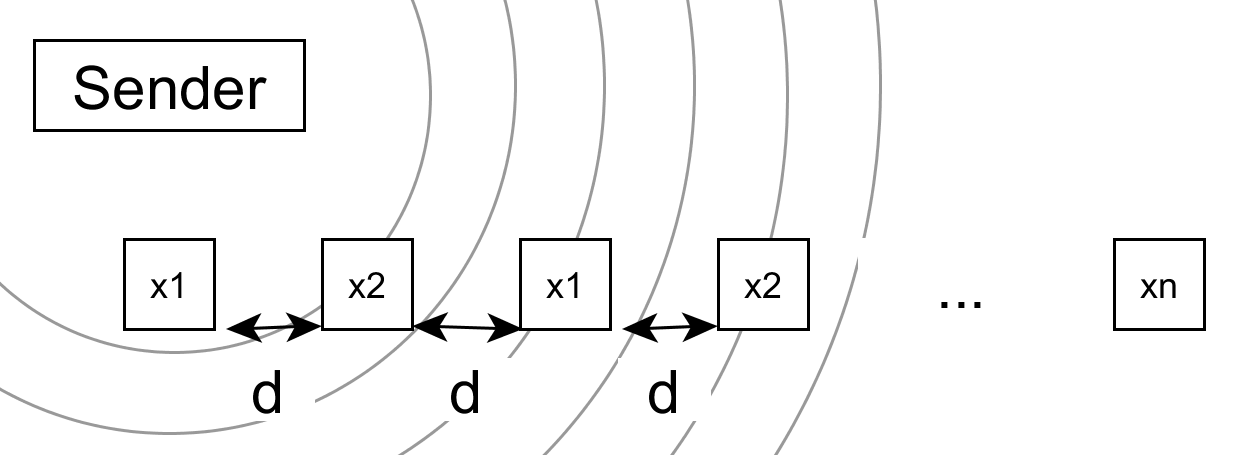
\includegraphics[scale=.27]{phase_int2.png}
\caption{Ankommende Wellenfronten an den Antennen}
\end{figure}

\section{Distanzbasierte Messung}
Im Folgenden werden Ansätze vorgestellt, welche den Abstand zwischen Sender und Empfänger ermitteln. Hierzu gehören \textit{Lighthouse approach}, \textit{\ac{TOA}}, \textit{Round-Trip Propagation} und \textit{\ac{TDOA}}.
  \subsection{Lighthouse Approach}
Das Verfahren, das dem \textit{Lighthouse approach}\cite{lighthouse} zugrunde liegt, basiert auf dem Prinzip eines Leuchtturms. Das Licht eines Lechtturms strahlt gerichtet und dreht sich um seine Achse, damit es von allen Seiten gesehen werden kann.\\
\indent
Für dieses Ortungsverfahren wird ein Sender benötigt, welcher als Leuchtturm fungiert. Die Empfänger des Signals müssen mit hoher Präzision arbeiten, also sollte das Licht des Senders ebenfalls möglichst ohne Abweichungen verlaufen. In {\bf Abb.3.2} ist der grobe Aufbau des \textit{Lighthouse approach} skizziert. Man kann erkennen, dass der Sender {\bf S} einen Strahl mit konstanter Breite {\bf b} ausstrahlt und sich um seine Achse dreht.\\

\begin{figure}[!htb]
\centering
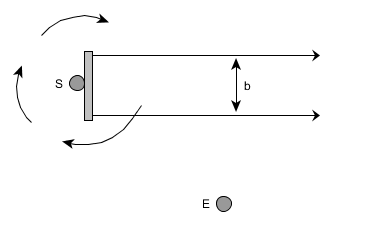
\includegraphics[scale=.68]{lighthouse.png}
\caption{Lighthouse Approach}
\end{figure}

Die Drehgeschwindigkeit des Senders ist vorher bekannt. Der Empfänger {\bf E} ist in Sichtweite aufgestellt und misst den Zeitunterschied zwischen dem Eintritt des Lichtsignals und dessen Austritt. Mithilfe der Drehgeschwindigkeit und der Zeit, die der Empfänger im Licht misst, kann die Entfernung berechnet werden.\\
\indent
Eine Möglichkeit, das Licht zu emittieren ist es, eine ausreichend breite parallele Lichtquelle zu nutzen. Parallel bedeutet, dass die Breite des Lichts unabhängig von der zurückgelegten Strecke möglichst konstant bleibt. Wie in \cite{lighthouse} beschrieben, ist dieses Vorgehen allerdings aufgrund von beschränkten Mitteln und Kapäzitäten der WSN Sensoren recht fehleranfällig und so wird z.B. ein 10cm breites Licht auf eine Entfernung von 5m eine Breite von 18.7cm erreichen.\\
\indent
Als Alternative ist es möglich, zwei Laser am Sender so anzubringen, dass sie einen in eine Richtung gerichteten, parallelen optischen Strahl simulieren. Mithilfe von vertikal und horizontal verstellbaren Spiegeln, an denen die Laser reflektiert werden, lassen sich feine Korrekturen an den Austrittswinkeln des Lichts vornehmen. Mit der \ac{COTS} Hardware lässt sich eine Drehfrequenz von bis zu 300Hz\cite{lighthouse} erreichen. 

  \subsection{One-Way Propagation}
\textit{One-Way Propagation} oder auch: \textit{\ac{TOA}} steht für die Übertragung eines Signals in eine Richtung\cite{toa}. Mithilfe der Übertragungszeit kann eine Distanz approximiert werden. Die Ausbreitungsgeschwindigkeit $c$\footnote{Lichtgeschwindigkeit} der Funkwellen ist bekannt. Diese Information lässt sich nutzen, um die Übertragungsdistanz zu errechnen. In der {\bf Abb. 3.3} sind 3 Anker und der Empfänger {\bf P} abgebildet. Die Radien aller 3 Anker schneiden sich in dem Punkt, an dem sich der Empfänger befinden soll.

\begin{figure}[!htb]
\centering
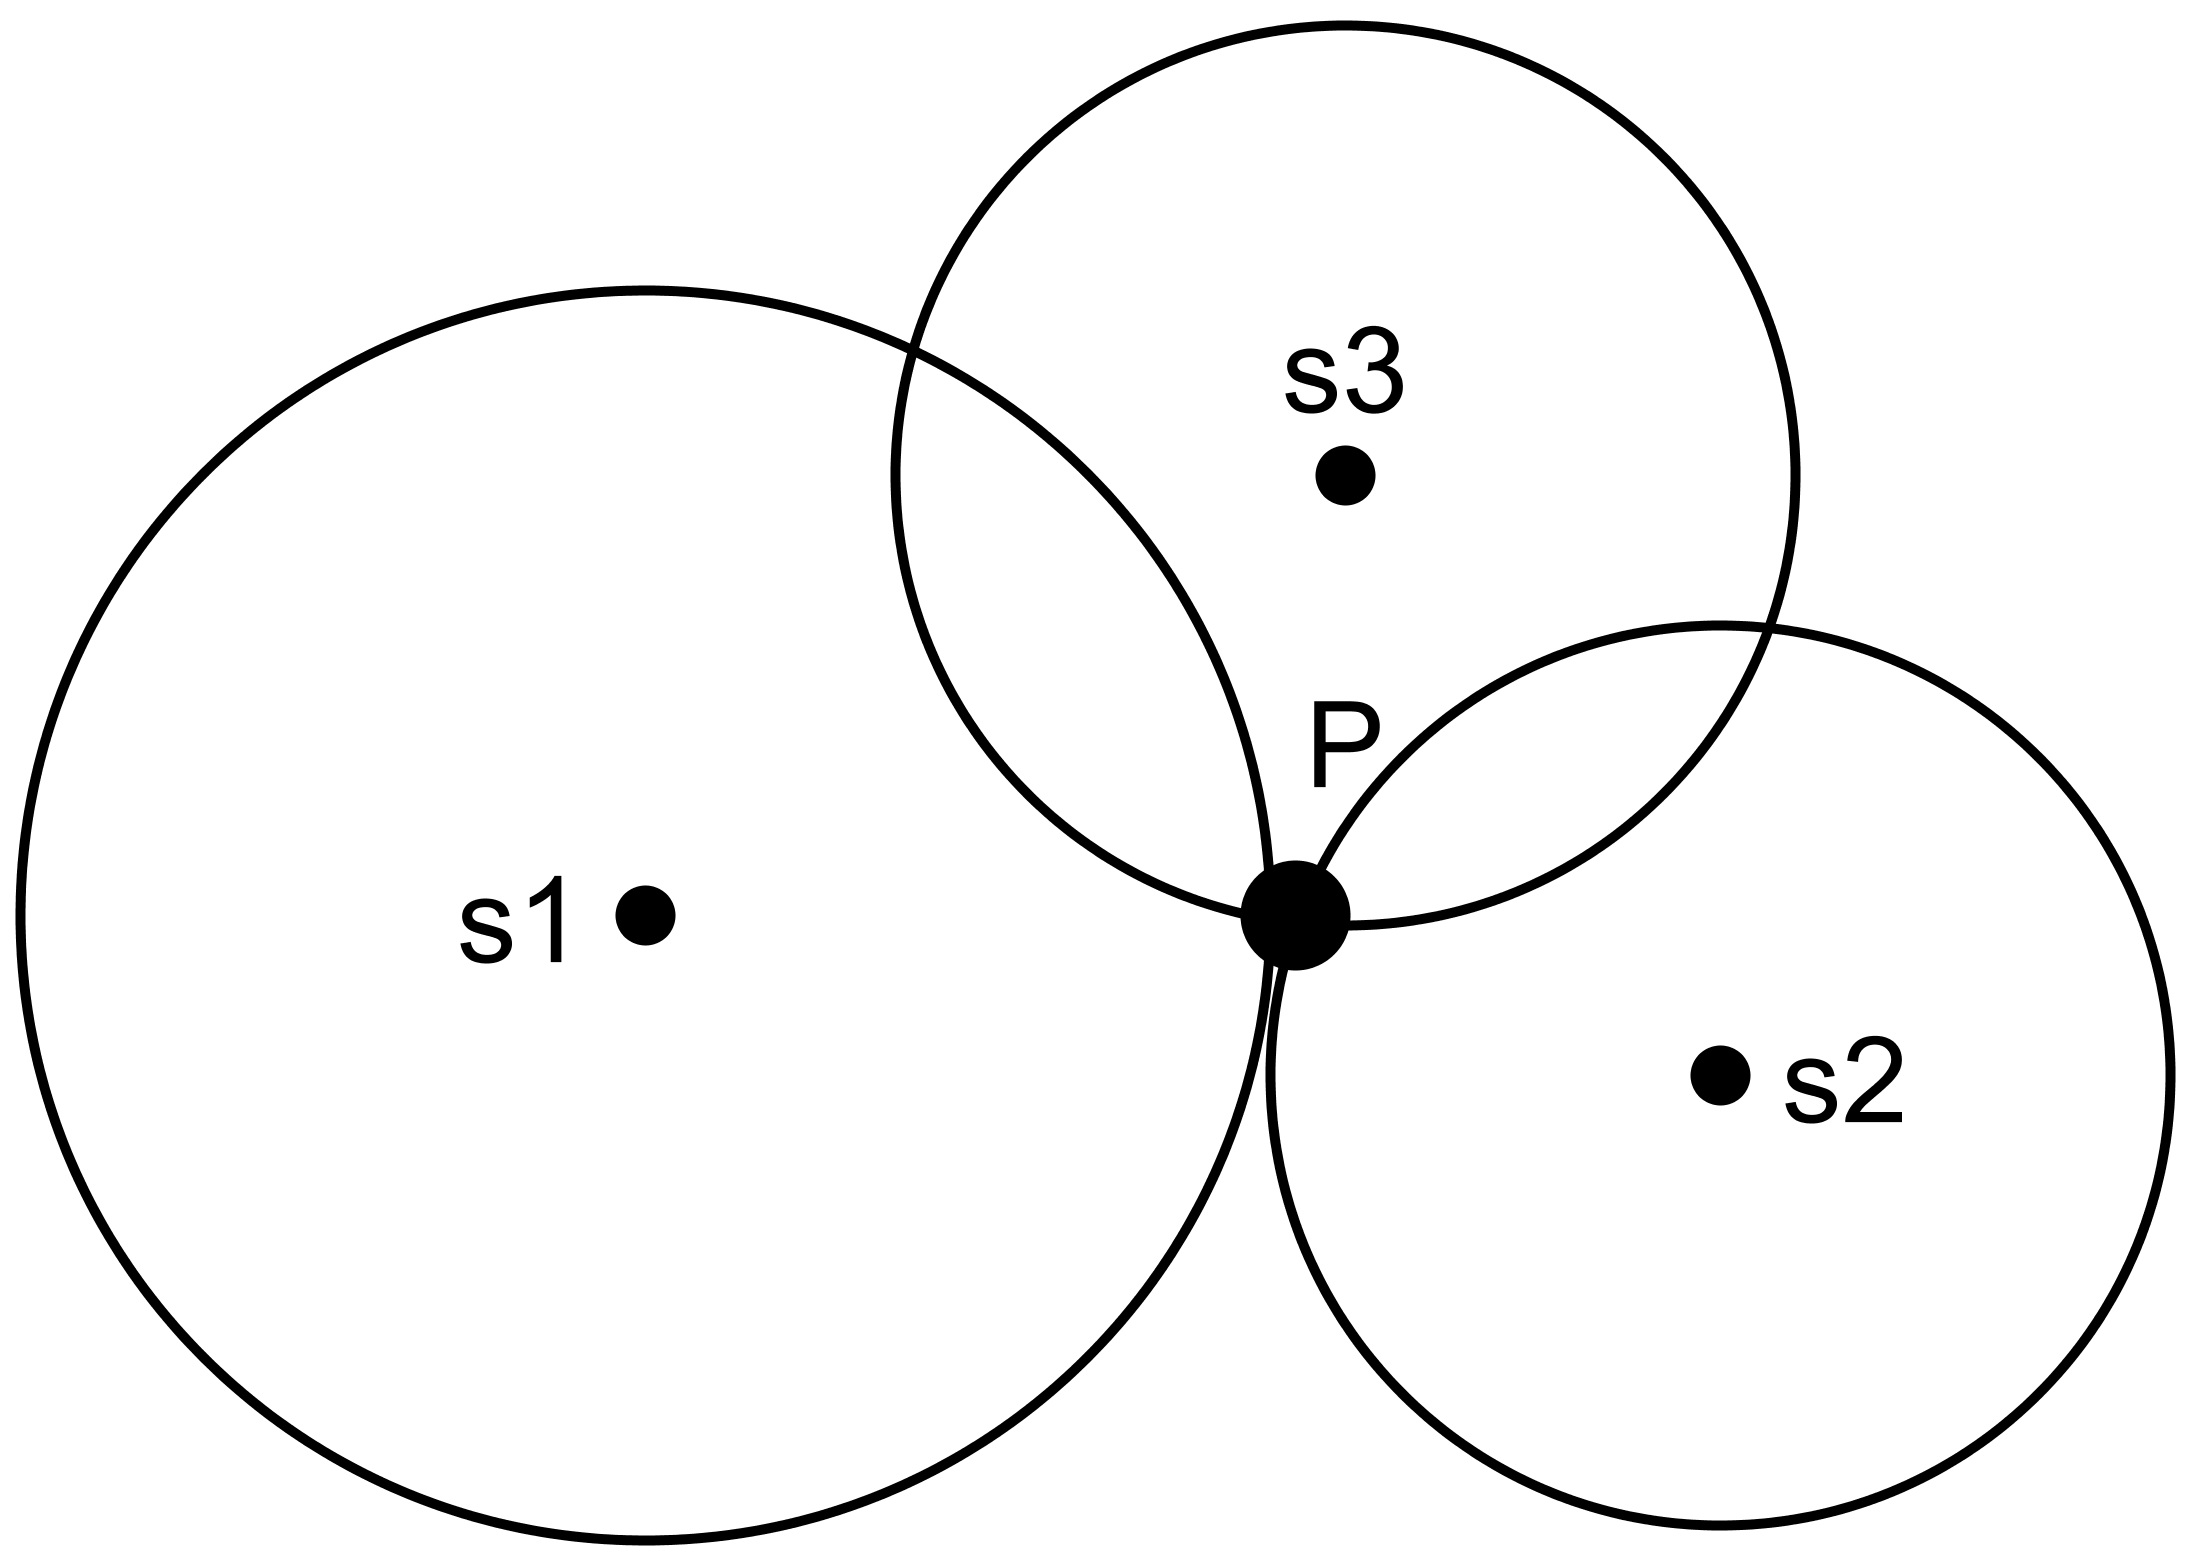
\includegraphics[scale=.07]{toa.png}
\caption{Zweidimensionale Lokalisierung mithilfe von TOA vgl.\cite{toa}}
\end{figure}

Man benötigt also mindestens 3 Anker, um die Position des Senders zu ermitteln. Der weitere wichtige Punkt ist die Synchronisierung der Geräte bezüglich der Uhren.
Um die Zeit zwischen dem Senden und Empfangen zu messen, muss der Empfänger die Uhrzeit des Sendens wissen. Die Uhr des Senders und die des Empfängers müssen also synchron laufen. Dies erfordert eine tiefere Kommunikation zwischen den Geräten, was die Komplexität der Hardware steigert. Das Vorgehen eignet sich also nicht besonders gut für \ac{WSN}, bei denen der Kostenfaktor minimal gehalten werden soll.

Eine mögliche Lösung zur Berechnung der Übertragungszeit wird in \cite{q1} erwähnt: Der Sender verschickt zusätzlich zum Radiosignal ein Ultraschallsignal. Das Radiosignal breitet sich mit $c$ aus und das Ultraschallsignal ist wesentlich langsamer. Der Empfänger horcht auf beide Signale und entsprechend der Differenz der Ankunftszeit kann die Übertragungsdauer berechnet werden. Allerdings steigt hierbei ebenfalls die Komplexität der Sensoren und das Vorgehen eignet sich nicht für Umgebungen mit ausgeprägtem potentiellen Mehrwegempfang. Mehr dazu in Kapitel 7. 

  \subsection{Time Difference Of Arrival}
Eine spezielle Abwandlung des \textit{\ac{TOA}}, welche mit Zeitdifferenzen eines ankommenden Signals arbeitet, ist die \textit{\ac{TDOA}}. Es werden mindestens 3 Anker benötigt, deren Positionen bekannt sind. Diese dienen als Empfänger für das ankommende Signal des zu lokalisierenden Senders. Sobald das Signal an allen Ankern angekommen ist, wird die Zeitdifferenz für die Lokalisierung genutzt. Diese Methode erfordert allerdings auch eine Synchronisierung der Ankeruhren.

  \subsection{Round-Trip Propagation}
Die erweiterte Alternative zur One-Way Propagation ist das \textit{ping} Prinzip. Hierbei wird das Signal nicht vom Empfänger gemessen. Stattdessen sendet der Empfänger das Signal wieder zurück und der ursprüngliche Sender vergleicht die Sende- und Rückkehrzeit des Signalpakets. Anhand dieser Zeitdifferenz lässt sich dann die Distanz berechnen. Hierbei wird keine Synchronisierung der Sender- und Empfängeruhren benötigt. Der Empfänger braucht allerdings eine bestimmte Zeit, um das Signal zu empfangen, verarbeiten und wieder zurückzuschicken. Diese Zeit kann der Empfänger selbst ausrechnen und zum Sender propagieren, damit die Berechnungen um diesen Wert korrigiert werden können.\\
    \subsection{RSS-basierte Lokalisierung}

\chapter{Range-free Methoden}
    \section{Flächenbasierte Lokalisierung}
Die flächenbasierte Lokalisierung ist eine Spezialform der \textit{range-free} Lokalisierungsansätze.

\chapter{Einsatzmöglichkeiten}
In der Einleitung wurden Beispiele für die Anwendungsbereiche der \acs{WSN} erwähnt. Bei dem ''precision farming'' werden Sensorknoten auf einem landwirtschaftlich genutzten Feld verteilt, damit sie die Luftfeuchtigkeit, Temperatur und Grundwasserspiegel messen können. Diese Messungen sollen die Produktivität der Ernte steigern.
\chapter{Aktuelle Probleme und Fragestellungen}
  \section{Multipath propagation}
\textit{Multipath propagation}(Mehrwegempfang) ist eines der Störfaktoren in der drahtlosen Übertragung. Dieser Faktor beeinflusst die Messungen, indem das Signal von Oberflächen reflektiert wird und somit ein gespiegeltes, schwächeres Signal entsteht. Dieses Phantomsignal kann als eine zusätzliche Quelle wahrgenommen werden kann.
  \section{Shadowing}

\chapter{Zusammenfassung}

\newpage
\bibliographystyle{IEEEtranN}
\bibliography{sources}
\nocite{*}
\end{document}